% triangular prism ABC-A1B1C1 with D on AB, E on BB1; dashed AC, DC, A1C
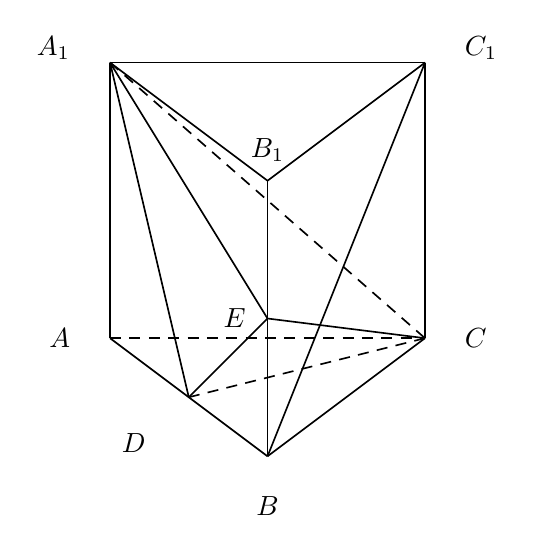
\begin{tikzpicture}[line width=0.6pt]
\coordinate (A1) at (0,5);
\coordinate (C1) at (4,5);
\coordinate (B1) at (2,3.5);
\coordinate (A) at (0,1.5);
\coordinate (C) at (4,1.5);
\coordinate (B) at (2,0);
\coordinate (D) at (1,0.75);
\coordinate (E) at (2,1.75);
\draw[draw=black] (A1)--(C1);
\draw[draw=black] (A1)--(A);
\draw[draw=black] (C1)--(C);
\draw[draw=black] (A1)--(B1)--(C1);
\draw[draw=black] (B1)--(B);
\draw[draw=black] (A)--(D)--(B);
\draw[draw=black] (B)--(C);
\draw[draw=black] (A1)--(D);
\draw[draw=black] (A1)--(E);
\draw[draw=black] (D)--(E)--(C);
\draw[draw=black] (B)--(C1);
\draw[draw=black,dash pattern=on 4pt off 3pt] (A)--(C);
\draw[draw=black,dash pattern=on 4pt off 3pt] (D)--(C);
\draw[draw=black,dash pattern=on 4pt off 3pt] (A1)--(C);
\node[anchor=east] at (-0.38,5.18) {$A_{1}$};
\node[anchor=west] at (4.38,5.18) {$C_{1}$};
\node[anchor=south] at (2,3.62) {$B_{1}$};
\node[anchor=east] at (-0.38,1.5) {$A$};
\node[anchor=west] at (4.38,1.5) {$C$};
\node[anchor=north] at (2,-0.38) {$B$};
\node[anchor=north east] at (0.58,0.42) {$D$};
\node[anchor=east] at (1.85,1.75) {$E$};
\end{tikzpicture}
